
\subsection{Answers}
\begin{table}[htb]%
\begin{center}%
\caption{Q25: If there were one communication aspect which is not enough in the current MPI could improve the performance of your application, what would you prioritize? Or is MPI providing all the communication semantics required by your application? If not, what is missing?}%
\label{tab:Q25-ans}%
\begin{tabular}{l|l|r}%
\hline%
Choice & Abbrv. & \# Answers \\%
\hline%
MPI provides all semantics I need & Satisfied & 174 (22.5\%) \\%
{\small Additional optimization opportunities in$\cdots$} & Additional comm. opt. & 150 (19.4\%) \\%
Multi-threading support & Multi-thread & 123 (15.9\%) \\%
{\small Optimization opportunities except commun$\cdots$} & Other opt & 99 (12.8\%) \\%
Latency & Latency & 98 (12.7\%) \\%
Bandwidth & Bandwidth & 62 (8.0\%) \\%
Message injection rate & Injection rate & 20 (2.6\%) \\%
Asynchronous progress & Asynch progress & 2 (0.3\%) \\%
other & - & 45 (5.8\%) \\%
\hline%
\multicolumn{2}{c}{total} & 773 \\%
\hline%
\end{tabular}%
\end{center}%
\end{table}%


In terms of optimization of the performance a small fraction of the users
are satisfied with the current situation. The main requirement concerns how MPI
provides general optimization opportunities in terms of communication such as
being able to handle the topology of the machine efficiently. Then comes how the
to handle multi-threading support which a prevalent issues in a world where a
lot of applications are run on multi-core nodes \mycomment[EJ]{here should cross
  Q22-Q25}. Other optimizations such as architecture awareness or dynamic
processing comes third. These issues are not related to the way MPI handles
communications but are identified as bottleneck for performance as well. Last
and interestingly almost twice as more users prioritize latency
optimization vs bandwidth optimization meaning that the overhead in starting to
send one message is seen as more prevalent than the time to send the message as
a whole. Region wise an interesting exception to this is Japan where much more
users ask for bandwidth optimization rather than
latency. 
\mycomment[EJ]{Does this means that Japan machines (K-computer?) have
  known issues in bandwidth or are already extremely good in latency?}
\mycomment[AH]{My guess is that they cannot distinguish bandwidth and
  injection rate.}

\subsection{List of other answers}
\begin{itemize}
\item Central and South America: I do not know if there is more to improve
\item Central and South America: dynamic scheduling
\item Europe:France: Energy consumption
\item Europe:France: I do not know
\item Europe:France: Mainly bandwidth and passing large arrays ~2GB+ memory usage and ofcourse the associated latency for large messages.
\item Europe:France: Much better error handling
\item Europe:France: RPC like API
\item Europe:France: asynchronous comm that are ACTUALLY asynchronous (that is to say, progress even when we're outside MPI)
\item Europe:France: dynamicity of nodes
\item Europe:France: injure that messages progresses while my code is computing (not only within MPI calls)
\item Europe:France: may be some control on the MPI overhead in massively parallel applications
\item Europe:France: platform interoperability (run-time)
\item Europe:France: rather than ibcast: isend same msg efficiently to several destinations, reception with irecv/recv. Or better (panel broadcast in a dense linear algebra factorizations): a way to pipeline communication and computation in an asynchronous broadcast tree. For example P0-\verb!>!(P1,P2);P1-\verb!>!(P3,P4), P2-\verb!>!(P5,P6), etc... while P3-P6 receive panel 1 (say), P1-P2  work with and forward panel 2, and P0 computes and sends panel 3, without synchronization and re-use of same buffer space for all panels
\item Europe:Germany: Exception handling
\item Europe:Germany: I don't know
\item Europe:Germany: I don't understand the question, we are fighting with latency and bandwidth
\item Europe:Germany: Latency for collective ops and bandwidth for point-to-point heavy codes.
\item Europe:Germany: Not fully aware of the issue
\item Europe:Germany: The first communication seems to be very slow with many MPI implementations (IBM MPI, Intel MPI,...)
\item Europe:Germany: ensure information from one-sided call (e.g. MPI\_Get) has arrived, without the need to close the communication fence (i.e. synchronize all ranks at once)
\item Europe:Germany: improve on one sided communication (GASPI, shmem style)
\item Europe:Italy: Interfacing with/switching from CUDA
\item Europe:UK: I don't know.
\item Europe:UK: MPI\_Comm\_ifree and similar would make life simpler. But most needed is something more subtle than MPI\_Abort for handling errors in applications. At the very least a portable way to make sure the error message actually gets to the user before the abort kicks in. To be clear I am NOT talking about errors within MPI, I am talking about MPI providing cleaner mechanisms to deal with application level errors
\item Europe:UK: More robust implementations
\item Europe:UK: Network congestion control
\item Europe:UK: The limit on data that can be sent and recieved using the pack / unpack , send / recv pattern. This is a severe limitation. My only way around it is to rewrite code to use my own custom datatypes, which seems unneccessarily complicated and time-consuming.
\item Europe:UK: Unsure
\item Europe:others: Fault tolerance/mitigation methods
\item Europe:others: I am thinking whether I will need HWLOC
\item Europe:others: I do not know
\item Europe:others: I sometimes want a feature which does not exist, at least in the most common implementations. An example would be MPI\_Recvreduce.
\item Europe:others: Unspecified message size
\item Europe:others: no clue
\item Japan: Fault Tolerancy
\item Japan: I don't know.
\item Japan: Slow initialization
\item Russia: Don't know
\item Russia: Too stupid to give an educated opinion
\item USA: Better passive-target MPI RMA performance. Better MPI\_THREAD\_MULTIPLE performance.
\item USA: Internal MPI statistics (off-node vs. on-node messages/bytes, etc.)
\item USA: Multi-threading support + Batching sends for better message injection rate
\item USA: Non-blocking collectives that could be used to loosen consistency semantics in PGAS languages
\item USA: RPC/Active messages support in MPI RMA (like UPC++ RPC). A public RPC API in RMA could be very useful for graph/combinatorial workloads.
\item USA: varies

\end{itemize}

\begin{figure}[htb]
\begin{center}
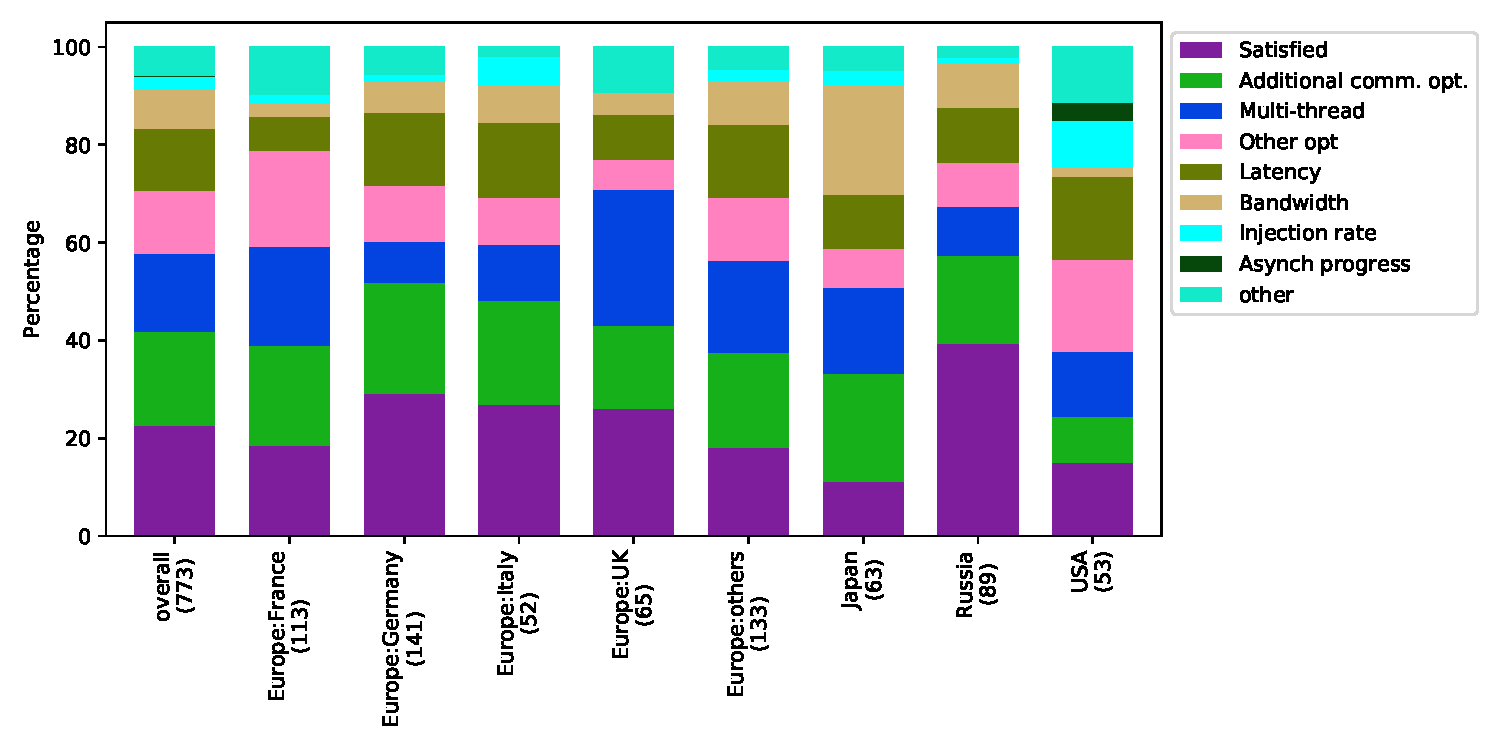
\includegraphics[width=10cm]{../pdfs/Q25.pdf}
\caption{Simple analysis: Q25}
\label{fig:Q25}
\end{center}
\end{figure}

\begin{figure}[htb]
\begin{center}
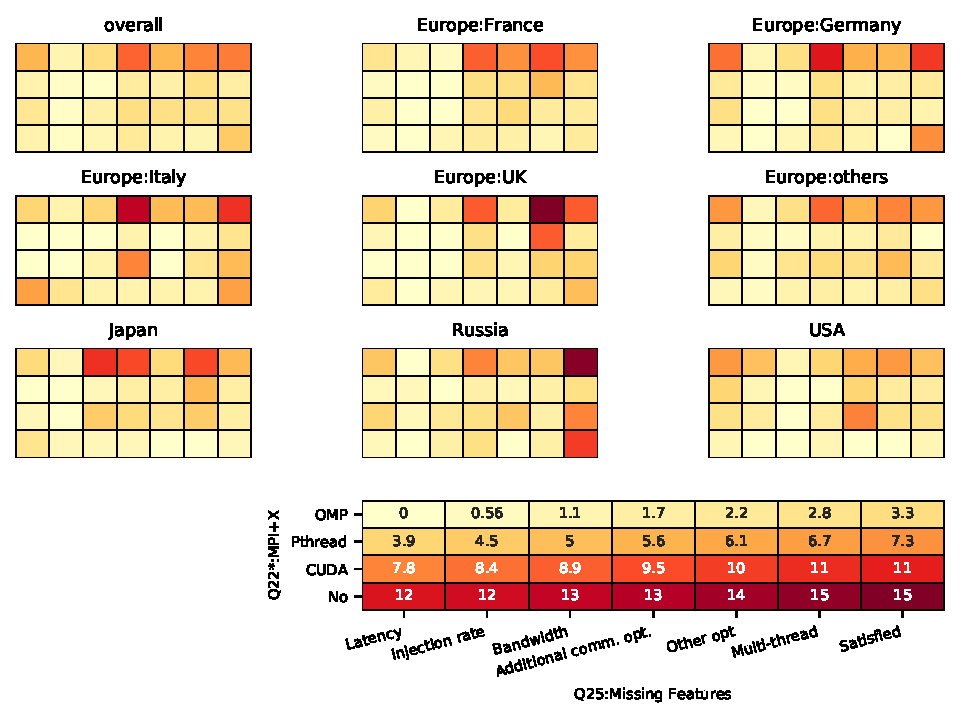
\includegraphics[width=10cm]{../pdfs/Q22-Q25.pdf}
\caption{Cross analysis: Q22-Q25}
\label{fig:Q25-and-Q22}
\end{center}
\end{figure}
